\documentclass[12pt]{article}

\usepackage{amsmath}
\usepackage{float}
\usepackage{graphicx}

\author{Andrew Mason \& Jon Pfeil}
\title{EECS 497 Programming Assignment 1}

\begin{document}
\maketitle

\begin{enumerate}
  \item
    The two models we implemented that required parameters were Laplace Smoothing
    and Absolute Discounting. For both of these models, we scaled the parameter and
    recorded the perplexity. For all of these, the Absolute Discounting model had
    a much lower perplexity than the Laplace Smoothing.\\
    \begin{figure}[H]
      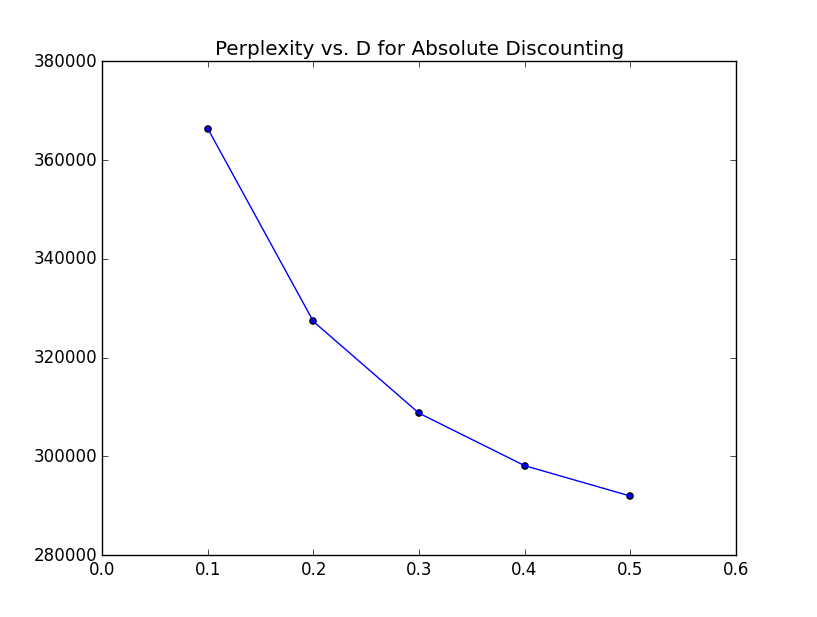
\includegraphics[width=\linewidth]{perplexity_vs_d.png}
    \end{figure}
    \begin{figure}[H]
      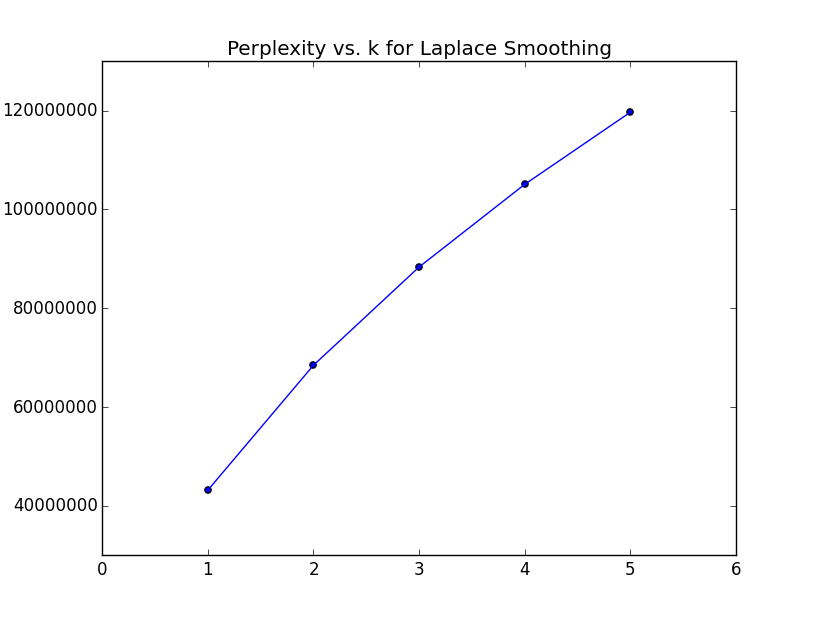
\includegraphics[width=\linewidth]{perplexity_vs_k.png}
    \end{figure}
  \item
    The corpus was easy to download and work with. We did not have any issues
    with the corpus other than it being a bit small. One nice usage we found
    was that we were able to use the corpus to do stemming on future test
    sets.\\
    We did not use any third-party libraries to do NLP tasks, since we were
    able to use the corpus to do stemming on the sentences we needed to
    unscramble, as noted above.\\
    One issue that we encountered was dealing with the products of very small
    ($10^{-15}$) probabilities when computing the perplexity. We decided to
    address this issue by using logs of probabilities. This then led to the
    following derivation, which reduced our risk of overflowing the products
    of the logs:\\
    \begin{equation}
      \begin{split}
        \text{Perplexity}&=\sqrt[N]{\prod_{i=1}^N\frac{1}{p(w_i|w_{i-1},\ldots,w_{i-K})}}\\
        \log\text{Perplexity}&=\log((\prod_{i=1}^N\frac{1}{p(w_i|w_{i-1},\ldots,w_{i-K})})^{\frac{1}{N}})\\
        &=\sum_{i=1}^N\frac{1}{N}\log(\frac{1}{p(w_i|w_{i-1},\ldots,w_{i-K})})\\
        &=\frac{1}{N}\sum_{i=1}^N\log(\frac{1}{p(w_i|w_{i-1},\ldots,w_{i-K})})\\
        &=-\frac{1}{N}\sum_{i=1}^N\log(p(w_i|w_{i-1},\ldots,w_{i-K}))\\
      \end{split}
    \end{equation}

    Then we could compute the log of the perplexity, and exponentiate to retreive
    the actual perpelexity.
\end{enumerate}
\end{document}
